\chapter{TỔNG QUAN VỀ CƠ SỞ LÝ THUYẾT}
\section{LƯỢC KHẢO TÀI LIỆU}  
\subsection{Nghiên cứu về Chatbot trong thương mại điện tử}
Chatbot là một trong những giải pháp công nghệ nổi bật, được ứng dụng rộng rãi nhằm tự động hóa giao tiếp giữa doanh nghiệp và khách hàng. Theo nhiều nghiên cứu gần đây, chatbot có thể thay thế một phần công việc của đội ngũ chăm sóc khách hàng, cung cấp dịch vụ 24/7, giảm tải chi phí vận hành và nâng cao trải nghiệm người dùng. Các nền tảng thương mại điện tử lớn như Amazon, Alibaba hay Shopee đều đã triển khai Chatbot để hỗ trợ tra cứu thông tin sản phẩm, xử lý đơn hàng và chăm sóc sau bán.  

Tại Việt Nam, nhiều doanh nghiệp nhỏ và vừa cũng đã bước đầu ứng dụng chatbot, đặc biệt trên các nền tảng mạng xã hội như Facebook Messenger. Tuy nhiên, việc khai thác chatbot trên các nền tảng bản địa, điển hình là Zalo, vẫn chưa được nghiên cứu và triển khai rộng rãi.  

\subsection{Nghiên cứu và ứng dụng Zalo Chatbot}
Zalo hiện là mạng xã hội có lượng người dùng lớn tại Việt Nam, với ưu thế mạnh mẽ trong giao tiếp và thương mại nội địa. Từ năm 2018, Zalo đã mở API cho phép phát triển chatbot, hỗ trợ doanh nghiệp xây dựng hệ thống tư vấn và chăm sóc khách hàng tự động. Một số nghiên cứu bước đầu cho thấy chatbot Zalo giúp doanh nghiệp Việt Nam tiếp cận khách hàng nhanh chóng hơn, đặc biệt trong các lĩnh vực bán lẻ, thương mại điện tử và dịch vụ công.  

Tuy vậy, phần lớn ứng dụng mới dừng lại ở các chức năng cơ bản như trả lời tin nhắn tự động hoặc gửi thông báo đơn hàng. Việc tích hợp sâu hơn chatbot Zalo với các hệ thống thương mại điện tử và công cụ marketing vẫn còn hạn chế, tạo ra khoảng trống cho các nghiên cứu và giải pháp ứng dụng thực tiễn.  

\subsection{Các nền tảng công nghệ hỗ trợ tự động hóa}
Song song với sự phát triển của chatbot, nhiều nền tảng hỗ trợ tự động hóa quy trình truyền thông và kinh doanh cũng được quan tâm. Các công cụ như \textbf{N8N} và \textbf{Make.com} cho phép xây dựng workflow tự động, liên kết nhiều ứng dụng với nhau (ví dụ: tạo nội dung $\rightarrow$ xử lý $\rightarrow$ đăng tải lên mạng xã hội). Trong khi đó, \textbf{WordPress} kết hợp với \textbf{WooCommerce} được sử dụng phổ biến để xây dựng website thương mại điện tử cho doanh nghiệp vừa và nhỏ nhờ tính dễ triển khai và chi phí thấp.  

Việc kết hợp các nền tảng này giúp doanh nghiệp tối ưu hóa toàn bộ chuỗi hoạt động: từ quản lý dữ liệu, tự động tạo nội dung, vận hành website, đến chăm sóc khách hàng thông qua chatbot.  

\subsection{Đánh giá và khoảng trống nghiên cứu}
Qua lược khảo, có thể thấy các nghiên cứu và ứng dụng hiện nay tập trung mạnh vào \textbf{chatbot trên Facebook Messenger} và các giải pháp thương mại điện tử truyền thống. Trong khi đó, \textbf{Zalo Chatbot}, một nền tảng có lợi thế tại thị trường Việt Nam, vẫn chưa được khai thác toàn diện. Bên cạnh đó, việc tích hợp đồng bộ \textbf{Chatbot Zalo – Website thương mại điện tử – Hệ thống tự động hóa truyền thông} chưa có nhiều nghiên cứu cụ thể.  

Chính vì vậy, đề tài ``\textit{Hệ thống Tự động hóa Truyền thông và Thương mại Điện tử cho Doanh nghiệp ứng dụng Chatbot Zalo}'' được thực hiện với mong muốn bổ sung vào khoảng trống này. Đề tài không chỉ mang ý nghĩa học thuật trong việc áp dụng công nghệ mới, mà còn có giá trị thực tiễn cao đối với doanh nghiệp vừa và nhỏ tại Việt Nam trong bối cảnh số hóa hiện nay.  

\section{CƠ SỞ LÝ THUYẾT}

\subsection{Google Sheets và Google Drive – nền tảng lưu trữ và quản lý dữ liệu trên đám mây}

\textbf{Định nghĩa:}
\begin{itemize}
    \item \textbf{Google Sheets} là ứng dụng bảng tính trực tuyến do Google phát triển, hoạt động trên nền tảng Web và đồng bộ với Google Drive. Sheets cho phép nhiều người dùng cùng tạo, chỉnh sửa và cộng tác trên một bảng tính theo thời gian thực.
    \item \textbf{Google Drive} là dịch vụ lưu trữ và đồng bộ tệp trên đám mây, cho phép tải lên, chia sẻ và truy cập tài liệu, hình ảnh, video từ bất kỳ thiết bị nào.
\end{itemize}

Trong hệ thống, Google Sheets được dùng để quản lý dữ liệu thương hiệu và sản phẩm, còn Google Drive lưu trữ hình ảnh/Video để Chatbot và hệ thống tự động hóa có thể sử dụng khi cần.

\textbf{Thành phần/Cấu trúc chính:}
\begin{itemize}
    \item \textbf{Google Sheets:}
    \begin{itemize}
        \item Cell/Row/Column: đơn vị cơ bản.
        \item Function \& Formula: tính toán, xử lý dữ liệu.
        \item Collaboration: nhiều người chỉnh sửa cùng lúc.
        \item Integration API: kết nối Make.com, N8N, AI.
    \end{itemize}
    \item \textbf{Google Drive:}
    \begin{itemize}
        \item File Storage: lưu nhiều định dạng.
        \item Folder Structure: tổ chức khoa học.
        \item Permission \& Sharing: quản lý quyền truy cập.
        \item API Access: ứng dụng có thể lấy/cập nhật dữ liệu.
    \end{itemize}
\end{itemize}

\textbf{Ứng dụng trong thực tiễn (KingPhone):}
\begin{itemize}
    \item Google Sheets: lưu thông tin thương hiệu, sản phẩm; nguồn dữ liệu đầu vào cho AI; kết nối với N8N để chatbot Zalo gửi Menu.
    \item Google Drive: lưu hình ảnh sản phẩm, Video Marketing để đăng tải lên YouTube, Fanpage.
\end{itemize}

\textbf{Ưu điểm:}
\begin{itemize}
    \item Miễn phí/chi phí thấp.
    \item Cộng tác theo thời gian thực.
    \item Tích hợp mạnh mẽ với API.
    \item Đồng bộ đám mây.
    \item Bảo mật với phân quyền chi tiết.
\end{itemize}

\textbf{Nhược điểm:}
\begin{itemize}
    \item Giới hạn dung lượng miễn phí (15GB).
    \item Phụ thuộc Internet.
    \item Bảo mật phụ thuộc người quản trị.
    \item Hiệu suất giảm khi dữ liệu lớn.
\end{itemize}

\textbf{Vai trò trong đề tài:}
\begin{itemize}
    \item Là nguồn dữ liệu trung tâm: Sheets cung cấp dữ liệu, Drive lưu media.
    \item Đảm bảo dữ liệu cập nhật và đồng bộ.
    \item Dễ quản lý, không cần can thiệp mã nguồn.
\end{itemize}

\textbf{Lợi ích:}
\begin{itemize}
    \item Kho dữ liệu linh hoạt, dễ chỉnh sửa.
    \item AI và Chatbot có thể tự động lấy dữ liệu mới nhất.
    \item Tạo sự kết nối chặt chẽ giữa Make.com – N8N – WordPress – Zalo – Fanpage – YouTube.
\end{itemize}

\begin{figure}
\centering
    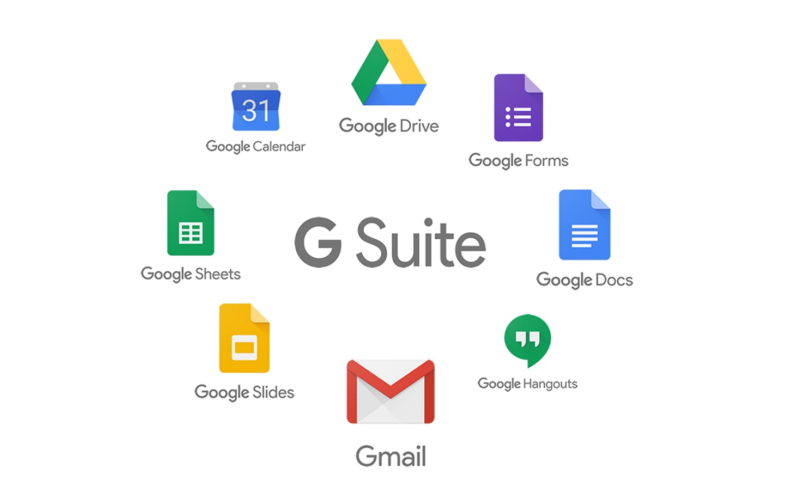
\includegraphics[width=0.7\textwidth]{img/gg.png}
    
    \caption{ Hệ sinh thái Google}
    \label{fig:gg}
\end{figure}


%----------------------------------------------------

\subsection{AI (Trí tuệ nhân tạo)}

\textbf{Định nghĩa:} AI là lĩnh vực khoa học máy tính phát triển hệ thống có khả năng mô phỏng trí tuệ con người (học hỏi, suy luận, giải quyết vấn đề, NLP, ra quyết định). Trong đề tài, AI được dùng để tạo nội dung Marketing và xử lý ngôn ngữ tự nhiên cho Chatbot Zalo.

\textbf{Thành phần/Cấu trúc chính:}
\begin{itemize}
    \item Natural Language Processing (NLP).
    \item Generative AI: sinh bài viết, hình ảnh, Video.
    \item Machine Learning Model: học dữ liệu từ Google Sheets.
    \item Integration With Workflow: kết nối Make.com, N8N.
\end{itemize}

\textbf{Ứng dụng:}
\begin{itemize}
    \item Make.com: sinh bài viết, ảnh, Video.
    \item N8N + Zalo API: phân tích tin nhắn, phản hồi tự động, gửi sản phẩm kèm hình ảnh.
\end{itemize}

\textbf{Ưu điểm:}
\begin{itemize}
    \item Tự động hóa sáng tạo nội dung.
    \item Hiểu ngôn ngữ tự nhiên.
    \item Tiết kiệm chi phí, thời gian.
    \item Khả năng mở rộng, linh hoạt.
\end{itemize}

\textbf{Nhược điểm:}
\begin{itemize}
    \item Chi phí API.
    \item Phụ thuộc dữ liệu huấn luyện.
    \item Hạn chế ngữ cảnh phức tạp.
    \item Cần giám sát nội dung sinh ra.
\end{itemize}

\textbf{Vai trò:}
\begin{itemize}
    \item Bộ não thông minh: Make.com sinh nội dung, N8N xử lý NLP cho chatbot.
    \item Đảm bảo hệ thống tự động và thông minh.
\end{itemize}

\textbf{Lợi ích:}
\begin{itemize}
    \item Hệ thống Marketing – chăm sóc khách hàng chuyên nghiệp.
    \item Trải nghiệm tư vấn 24/7.
    \item Nội dung đồng bộ thương hiệu.
\end{itemize}

\begin{figure}
\centering
    
\includegraphics[width=0.8\textwidth]{img/Picture2.png}
    
    \caption{Mô hình AI trong chăm sóc khách hàng}
    \label{fig:chamsoc}
\end{figure}

%----------------------------------------------------

\subsection{Zalo API qua N8N – tích hợp Chatbot}

\textbf{Định nghĩa:} Zalo API được tích hợp qua N8N để giảm độ phức tạp và tăng linh hoạt, phục vụ xây dựng chatbot thương mại điện tử.

\textbf{Thành phần:}
\begin{itemize}
    \item Webhook Trigger Node.
    \item Message Node.
    \item User Node.
    \item Google Sheets/Drive Node.
    \item AI Node (OpenAI).
    \item Database Node.
    \item Admin Flow.
\end{itemize}

\textbf{Ứng dụng (KingPhone):}
\begin{itemize}
    \item Tiếp nhận, phân loại tin nhắn.
    \item Cung cấp menu sản phẩm động.
    \item Tư vấn tự động 24/7.
    \item Đồng bộ với Website TMĐT.
    \item Hỗ trợ quản trị viên.
\end{itemize}

\textbf{Ưu điểm:}
\begin{itemize}
    \item Tích hợp dễ dàng.
    \item Linh hoạt.
    \item Tự động hóa mạnh.
    \item Dữ liệu tập trung.
    \item Phù hợp thị trường Việt Nam.
\end{itemize}

\textbf{Nhược điểm:}
\begin{itemize}
    \item Yêu cầu kỹ năng N8N.
    \item Phụ thuộc Server.
    \item Cần bảo mật tốt Token, dữ liệu.
\end{itemize}

\begin{figure}
    \centering
    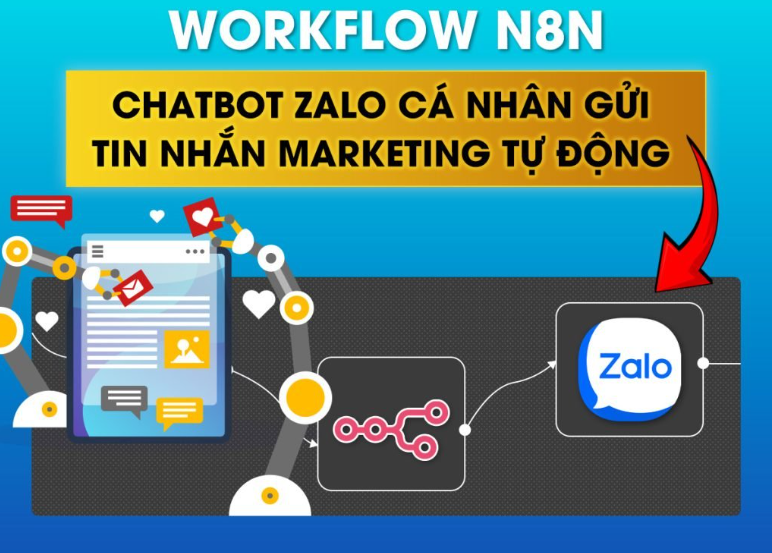
\includegraphics[width=0.7\textwidth]{img/Picture3.png}

    \caption{Zalo API qua N8N trong hệ thống tư vấn khách hàng}
    \label{fig:zaloapi}
\end{figure}

%----------------------------------------------------

\subsection{Make.com – nền tảng tự động hóa quy trình}

\textbf{Định nghĩa:} Make.com (trước đây Integromat) là nền tảng Automation, kết nối ứng dụng, dịch vụ, API bằng giao diện kéo-thả, không cần nhiều Code.

\textbf{Thành phần:}
\begin{itemize}
    \item Scenario.
    \item Module.
    \item Trigger.
    \item Action.
    \item Iterator \& Aggregator.
    \item Error Handler.
\end{itemize}

\textbf{Ứng dụng (KingPhone):}
\begin{itemize}
    \item Sheets nhập dữ liệu thương hiệu.
    \item AI sinh nội dung.
    \item Drive lưu Media.
    \item WordPress, Facebook, YouTube đăng bài.
\end{itemize}

\textbf{Ưu điểm:}
\begin{itemize}
    \item Không cần lập trình nhiều.
    \item Tích hợp linh hoạt.
    \item Tự động hóa mạnh.
    \item Khả năng mở rộng.
    \item Tiết kiệm chi phí.
\end{itemize}

\textbf{Nhược điểm:}
\begin{itemize}
    \item Phụ thuộc Internet.
    \item Thiết lập Workflow phức tạp.
    \item Giới hạn theo gói dịch vụ.
    \item Bảo mật phụ thuộc Cloud.
\end{itemize}

\begin{figure}
\centering
    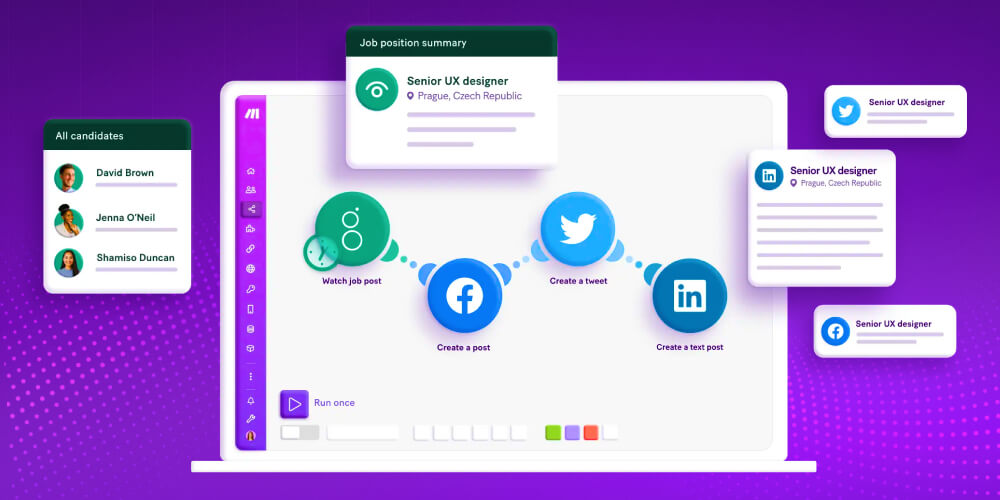
\includegraphics[width=0.8\textwidth]{img/Picture4.png}

    \caption{Make.com}
    \label{fig:make}
\end{figure}

%----------------------------------------------------

\subsection{N8N – nền tảng mã nguồn mở}

\textbf{Định nghĩa:} N8N là nền tảng Automation mã nguồn mở, có thể Self-hosted, đảm bảo bảo mật và tùy biến cao.

\textbf{Thành phần:}
\begin{itemize}
    \item Workflow.
    \item Node.
    \item Trigger Node.
    \item Action Node.
    \item Credential Management.
    \item Database Storage.
    \item Error Workflow.
\end{itemize}

\textbf{Ứng dụng (KingPhone):}
\begin{itemize}
    \item Nhận tin nhắn khách hàng.
    \item Phân loại tin nhắn.
    \item AI phân tích, phản hồi.
    \item Kết nối Sheets/Drive gửi sản phẩm.
    \item Lưu trữ hội thoại.
    \item Quản trị viên kiểm soát.
\end{itemize}

\textbf{Ưu điểm:}
\begin{itemize}
    \item Mã nguồn mở, tự triển khai.
    \item Tùy biến cao.
    \item Chi phí thấp.
    \item Tích hợp AI, API mạnh.
    \item Cộng đồng phát triển năng động.
\end{itemize}

\textbf{Nhược điểm:}
\begin{itemize}
    \item Yêu cầu kiến thức kỹ thuật.
    \item Cần hạ tầng riêng.
    \item Độ phức tạp ban đầu cao.
    \item Hiệu năng phụ thuộc Server.
\end{itemize}

\begin{figure}
\centering
    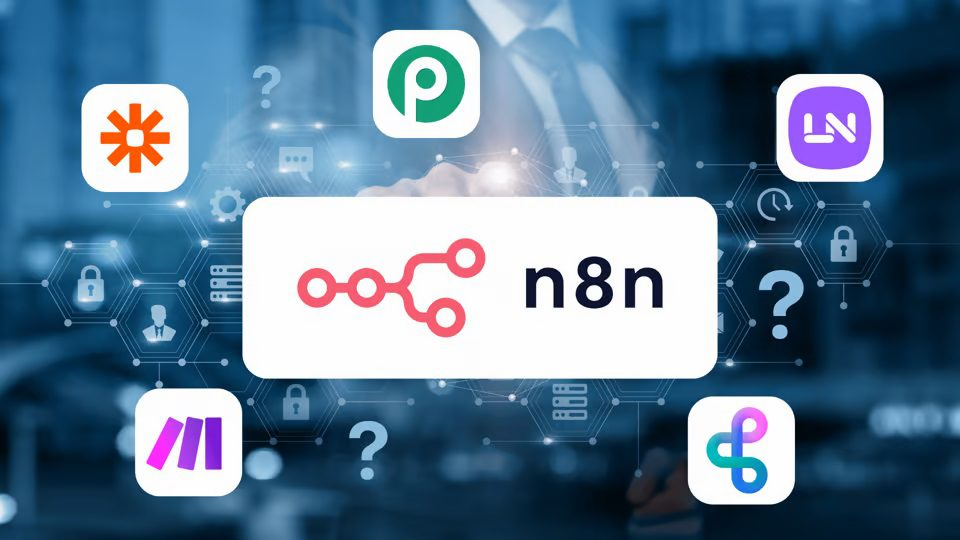
\includegraphics[width=0.8\textwidth]{img/Picture5.png}

    \caption{ N8N}
    \label{fig:n8n}
\end{figure}

%----------------------------------------------------

\subsection{WordPress và WooCommerce – nền tảng xây dựng Website thương mại điện tử}

\textbf{Định nghĩa}
WordPress là một hệ quản trị nội dung (CMS – Content Management System) mã nguồn mở, được phát triển từ năm 2003 và hiện là nền tảng Website phổ biến nhất thế giới. Ban đầu WordPress chủ yếu phục vụ viết Blog, nhưng ngày nay đã phát triển thành một nền tảng linh hoạt cho đủ loại Website: tin tức, giáo dục, thương mại điện tử, doanh nghiệp\dots

WooCommerce là một Plugin thương mại điện tử dành cho WordPress, ra mắt năm 2011, cho phép biến Website WordPress thành một cửa hàng trực tuyến đầy đủ chức năng: quản lý sản phẩm, giỏ hàng, thanh toán, đơn hàng, khách hàng. WooCommerce hiện chiếm hơn 25\% các Website thương mại điện tử trên toàn cầu.

\textbf{Thành phần/Cấu trúc}
\begin{itemize}
    \item \textbf{WordPress Core}: Phần lõi mã nguồn mở, cung cấp chức năng quản lý trang, bài viết, người dùng, Media.
    \item \textbf{Theme}: Giao diện Website, có thể tùy chỉnh hoặc cài đặt theme có sẵn để thay đổi thiết kế.
    \item \textbf{Plugin}: Các phần mở rộng bổ sung chức năng, ví dụ: SEO, bảo mật, Livechat, quản lý vận chuyển.
    \item \textbf{WooCommerce}: Plugin cốt lõi để bán hàng, bao gồm:
    \begin{itemize}
        \item Quản lý sản phẩm (thêm, sửa, xóa, phân loại).
        \item Giỏ hàng và thanh toán.
        \item Quản lý đơn hàng, khách hàng.
        \item Tích hợp thanh toán Online, vận chuyển.
    \end{itemize}
    \item \textbf{Database (MySQL/MariaDB)}: Lưu trữ dữ liệu sản phẩm, khách hàng, đơn hàng, cài đặt hệ thống.
\end{itemize}

\textbf{Ứng dụng trong thực tiễn}
Trong đề tài, WordPress + WooCommerce được sử dụng để xây dựng Website bán điện thoại KingPhone:
\begin{itemize}
    \item Hiển thị sản phẩm (IPhone các đời, thông tin, giá bán, hình ảnh).
    \item Cho phép khách hàng thêm sản phẩm vào giỏ, thanh toán trực tuyến.
    \item Quản lý đơn hàng, trạng thái giao dịch.
    \item Tích hợp Plugin SEO (Rank Math SEO) để tối ưu tìm kiếm.
    \item Hỗ trợ Livechat, liên kết với Chatbot Zalo.
    \item Là trung tâm kết nối với hệ thống Make.com.
\end{itemize}


\textbf{Ưu điểm:}
\begin{itemize}
    \item Mã nguồn mở, miễn phí.
    \item Cộng đồng lớn, kho Plugin và Theme phong phú.
    \item Tùy biến linh hoạt, từ Blog nhỏ đến Website lớn.
    \item Thân thiện SEO.
    \item Tích hợp dễ dàng với API, Chatbot, công cụ Automation.
\end{itemize}

\textbf{Nhược điểm:}
\begin{itemize}
    \item Hiệu suất phụ thuộc Plugin.
    \item Bảo mật cần quản lý thường xuyên.
    \item Cần kiến thức kỹ thuật về Server và Database.
    \item Chi phí Hosting cho TMĐT cao hơn so với Blog thông thường.
\end{itemize}

\textbf{Vai trò trong đề tài}
\begin{itemize}
    \item Cửa hàng trực tuyến trung tâm: nơi khách hàng xem và mua điện thoại.
    \item Quản lý đơn hàng, sản phẩm, khách hàng.
    \item Nhận nội dung Marketing tự động từ Make.com.
    \item Kết nối với Chatbot Zalo để hỗ trợ khách hàng.
\end{itemize}

\textbf{Lợi ích:}  
Giúp xây dựng cửa hàng Online chuyên nghiệp, tối ưu quy trình mua bán, và kết hợp với Automation để hình thành một hệ sinh thái số.

Theo số liệu W3Techs 2023, hơn 43\% Website toàn cầu sử dụng WordPress, và WooCommerce là nền tảng thương mại điện tử phổ biến nhất.

\begin{figure}[h!]
    \centering
    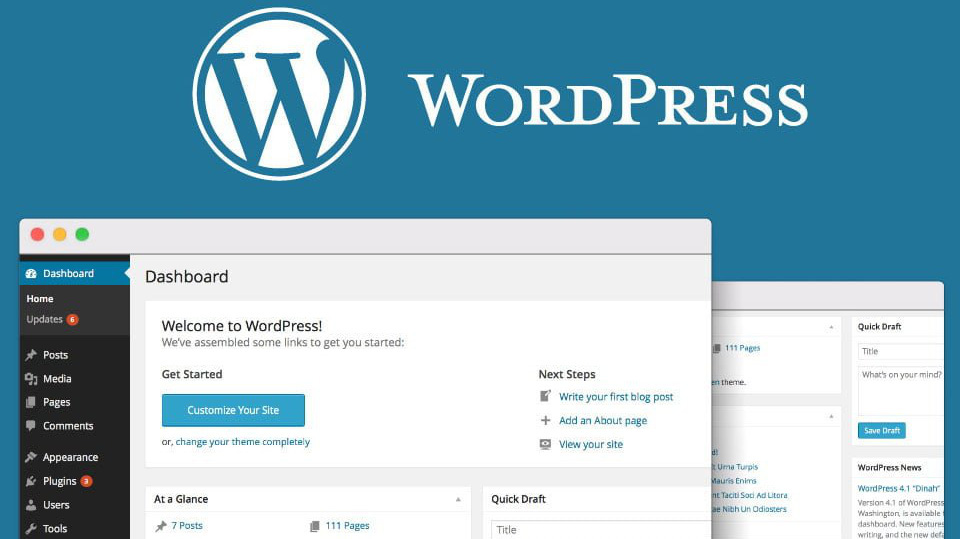
\includegraphics[width=0.75\textwidth]{img/Picture6.png}

    \caption{ Giao diện quản trị WordPress WooCommerce}
    \label{fig:wordpress}
\end{figure}

%---------------------------

\subsection{Facebook Fanpage và YouTube – kênh truyền thông và phân phối nội dung số}

\textbf{Định nghĩa}
\begin{itemize}
    \item \textbf{Facebook Fanpage}: Trang chính thức trên Facebook dành cho doanh nghiệp, thương hiệu hoặc cộng đồng, cho phép đăng tải bài viết, hình ảnh, video, tương tác trực tiếp qua bình luận, tin nhắn.
    \item \textbf{YouTube}: Nền tảng chia sẻ video lớn nhất thế giới, cho phép doanh nghiệp xây dựng kênh chính thức để đăng tải Video giới thiệu sản phẩm, hướng dẫn sử dụng, quảng cáo.
\end{itemize}

\textbf{Thành phần/Cấu trúc}
\textbf{Facebook Fanpage:}
\begin{itemize}
    \item Bài viết (Posts).
    \item Video/Live Stream.
    \item Messenger Chat.
    \item Insight \& Analytics.
\end{itemize}

\textbf{YouTube Channel:}
\begin{itemize}
    \item Video Uploads.
    \item Playlist.
    \item Comment \& Interaction.
    \item YouTube Studio.
\end{itemize}

\textbf{Ứng dụng trong thực tiễn}
\begin{itemize}
    \item Tích hợp Make.com để đăng nội dung tự động.
    \item Fanpage tiếp cận và chăm sóc khách hàng.
    \item YouTube tạo thư viện video marketing dài hạn.
\end{itemize}


\textbf{Ưu điểm:}
\begin{itemize}
    \item Tiếp cận khách hàng lớn.
    \item Đa dạng nội dung: văn bản, hình ảnh, Video, Livestream.
    \item Tăng tương tác, hỗ trợ quảng cáo.
    \item Công cụ phân tích chi tiết.
\end{itemize}

\textbf{Nhược điểm:}
\begin{itemize}
    \item Cạnh tranh cao.
    \item Phụ thuộc thuật toán.
    \item Cần duy trì thường xuyên.
\end{itemize}

\textbf{Vai trò trong đề tài}
\begin{itemize}
    \item \textbf{Facebook Fanpage}: Kênh Marketing chính, đăng tải Video quảng cáo tự động.
    \item \textbf{YouTube}: Kênh truyền thông bổ trợ, lưu trữ Video dài hạn, tăng độ tin cậy thương hiệu.
\end{itemize}

\begin{figure}[h!]
    \centering
    
\includegraphics[width=0.75\textwidth]{img/Picture7.png}
    
    \caption{ Fanpage Facebook và YouTube Channel}
    \label{fig:fb-yt}
\end{figure}

%---------------------------

\subsection{Supabase – nền tảng cơ sở dữ liệu và Backend mã nguồn mở}

\textbf{Định nghĩa}
Supabase là một nền tảng Backend-as-a-Service (BaaS) mã nguồn mở, dựa trên PostgreSQL. Nó cung cấp Real-time database, API tự động sinh, Authentication, Storage và Serverless Functions.
\begin{figure}[h!]
    \centering
    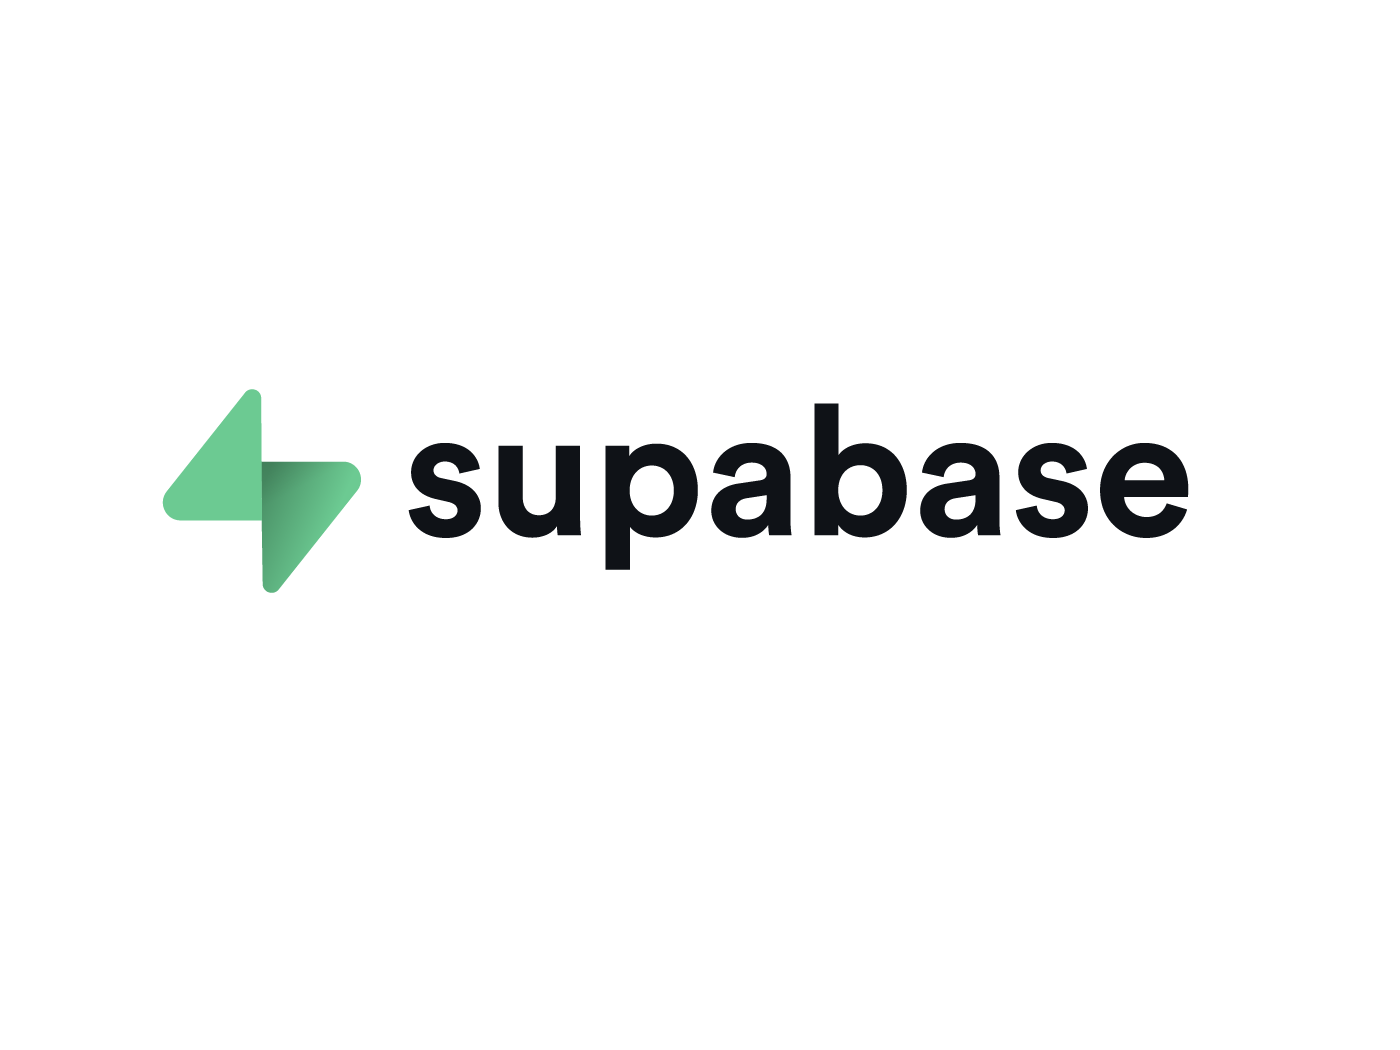
\includegraphics[width=0.75\textwidth]{img/Picture8.png}
    
    \caption{Supabase}
    \label{fig:supabase}
\end{figure}
\textbf{Thành phần/Cấu trúc}
\begin{itemize}
    \item PostgreSQL Database.
    \item Supabase API (RESTful \& GraphQL).
    \item Authentication.
    \item Realtime.
    \item Storage.
    \item Edge Functions.
    \item Dashboard.
\end{itemize}

\textbf{Ứng dụng trong thực tiễn}
\begin{itemize}
    \item Lưu trữ khách hàng, sản phẩm, đơn hàng.
    \item Đồng bộ dữ liệu Real-time.
    \item Quản lý xác thực người dùng.
    \item Lưu file (ảnh, Video).
    \item Xử lý nghiệp vụ bằng Edge Functions.
\end{itemize}


\textbf{Ưu điểm:} Mã nguồn mở, API tự động, Realtime mạnh, bảo mật cao, chi phí hợp lý. 

\textbf{Nhược điểm:} Đang phát triển, cần kiến thức PostgreSQL, hiệu năng phụ thuộc hạ tầng, cộng đồng nhỏ hơn Firebase.

\textbf{Vai trò trong đề tài}
\begin{itemize}
    \item Thay thế/bổ sung Google Sheets/Drive.
    \item Lưu trữ dữ liệu sản phẩm, khách hàng.
    \item Quản lý xác thực.
    \item Tích hợp N8N/Make.com qua API.
\end{itemize}



%---------------------------

\subsection{PostgreSQL – hệ quản trị cơ sở dữ liệu quan hệ mã nguồn mở}

\textbf{Định nghĩa}
PostgreSQL (Postgres) là hệ quản trị cơ sở dữ liệu quan hệ (RDBMS) mã nguồn mở, phát triển từ 1986 tại Đại học California, Berkeley. Nó nổi bật nhờ khả năng lưu trữ dữ liệu quan hệ, hỗ trợ JSON, XML, GIS\dots

\begin{figure}[h!]
    \centering
    
\includegraphics[width=0.65\textwidth]{img/Picture9.png}
    
    \caption{ PostgreSQL}
    \label{fig:postgresSLQ}
\end{figure}

\textbf{Thành phần/Cấu trúc}
\begin{itemize}
    \item Database Cluster.
    \item Database.
    \item Schema.
    \item Table.
    \item Data Types.
    \item Query Engine.
    \item Index.
    \item Transaction \& ACID.
    \item Replication.
\end{itemize}

\textbf{Ứng dụng trong thực tiễn}
\begin{itemize}
    \item Web và ứng dụng TMĐT.
    \item Chatbot \& Automation.
    \item Phân tích dữ liệu.
    \item GIS với PostGIS.
    \item Backend hiện đại (Supabase, Hasura).
\end{itemize}

\textbf{Ưu điểm:} Mã nguồn mở, chuẩn SQL, mở rộng mạnh, ổn định và bảo mật, replication tốt. 

\textbf{Nhược điểm:} Cần kỹ năng quản trị, hiệu năng thấp hơn NoSQL ở dữ liệu phi cấu trúc, khó tối ưu Big Data.

\textbf{Vai trò trong đề tài}
\begin{itemize}
    \item Lưu trữ dữ liệu sản phẩm, khách hàng, đơn hàng.
    \item Hỗ trợ Chatbot và Website.
    \item Thay thế Google Sheets khi cần Database chuyên nghiệp.
    
\end{itemize}

\\
\section{KẾT QUẢ NGHIÊN CỨU TRONG VÀ NGOÀI NƯỚC CÓ LIÊN QUAN}
\subsection{Kết quả nghiên cứu trong nước}
Tại Việt Nam, nhiều nghiên cứu tập trung vào việc áp dụng Chatbot trong các lĩnh vực thương mại điện tử, giáo dục, và dịch vụ công. Các đề tài này nhấn mạnh khả năng:
\begin{itemize}
    \item Hỗ trợ tự động tư vấn khách hàng, tiết kiệm thời gian và chi phí nhân sự.
    \item Ứng dụng Chatbot trong quảng bá sản phẩm, bán hàng trực tuyến.
    \item Nâng cao trải nghiệm khách hàng nhờ phản hồi nhanh chóng và chính xác.
\end{itemize}

Các nghiên cứu thực nghiệm cũng cho thấy việc ứng dụng Chatbot Zalo có tiềm năng lớn vì đây là nền tảng có số lượng người dùng cao tại Việt Nam, phù hợp cho doanh nghiệp vừa và nhỏ.

\subsection{Kết quả nghiên cứu ngoài nước}
Trên thế giới, nhiều công trình khoa học đã khẳng định hiệu quả của Chatbot trong thương mại điện tử và marketing số. Một số xu hướng nổi bật:
\begin{itemize}
    \item Chatbot ứng dụng trí tuệ nhân tạo (AI) và xử lý ngôn ngữ tự nhiên (NLP) để hiểu ngữ cảnh và cải thiện độ chính xác khi giao tiếp.
    \item Kết hợp Chatbot với hệ thống quản lý khách hàng (CRM) giúp cá nhân hóa dịch vụ.
    \item Ứng dụng Chatbot trong đa dạng lĩnh vực như chăm sóc y tế, tài chính, giáo dục và thương mại.
\end{itemize}

Các nghiên cứu ngoài nước cũng chỉ ra rằng Chatbot không chỉ dừng ở việc trả lời tự động, mà còn là công cụ thu thập dữ liệu, phân tích hành vi khách hàng và đưa ra gợi ý sản phẩm phù hợp. Điều này mở ra triển vọng lớn cho các doanh nghiệp trong việc tối ưu hóa chiến lược kinh doanh.


